%!TEX program = xelatex

\documentclass[a4paper, openany, oneside]{memoir}
\usepackage[no-math]{fontspec}
\usepackage{pgfplots}
\pgfplotsset{compat=newest}
\usepackage{commath}
\usepackage{mathtools}
\usepackage{amssymb}
\usepackage{amsthm}
\usepackage{booktabs}
\usepackage{mathtools}
\usepackage{xcolor}
\usepackage[separate-uncertainty=true, per-mode=symbol]{siunitx}
\usepackage[noabbrev, capitalize]{cleveref}
\usepackage{listings}
\usepackage[american inductor, european resistor]{circuitikz}
\usepackage{amsmath}
\usepackage{amsfonts}
\usepackage{ifxetex}
\usepackage[dutch,english]{babel}
\usepackage[backend=bibtexu,texencoding=utf8,bibencoding=utf8,style=ieee,sortlocale=en_GB,language=auto]{biblatex}
\usepackage[strict,autostyle]{csquotes}
\usepackage{parskip}
\usepackage{import}
\usepackage{standalone}
\usepackage{hyperref}
%\usepackage[toc,title,titletoc]{appendix}

\ifxetex{} % Fonts laden in het geval dat je met Xetex compiled
    \usepackage{fontspec}
    \defaultfontfeatures{Ligatures=TeX} % To support LaTeX quoting style
    \setromanfont{Palatino Linotype} % Tover ergens in Font mapje in root.
    \setmonofont{Source Code Pro}
\else % Terug val in standaard pdflatex tool chain. Geen ondersteuning voor OTT fonts
    \usepackage[T1]{fontenc}
    \usepackage[utf8]{inputenc}
\fi
\newcommand{\references}[1]{\begin{flushright}{#1}\end{flushright}}
\renewcommand{\vec}[1]{\boldsymbol{\mathbf{#1}}}
\newcommand{\uvec}[1]{\boldsymbol{\hat{\vec{#1}}}}
\newcommand{\mat}[1]{\boldsymbol{\mathbf{#1}}}
\newcommand{\fasor}[1]{\boldsymbol{\tilde{\vec{#1}}}}
\newcommand{\cmplx}[0]{\mathrm{j}}
\renewcommand{\Re}[0]{\operatorname{Re}}
\newcommand{\Cov}{\operatorname{Cov}}
\newcommand{\Var}{\operatorname{Var}}
\newcommand{\proj}{\operatorname{proj}}
\newcommand{\Perp}{\operatorname{perp}}
\newcommand{\col}{\operatorname{col}}
\newcommand{\rect}{\operatorname{rect}}
\newcommand{\sinc}{\operatorname{sinc}}
\newcommand{\IT}{\operatorname{IT}}
\newcommand{\F}{\mathcal{F}}

\newtheorem{definition}{Definition}
\newtheorem{theorem}{Theorem}


\DeclareSIUnit{\voltampere}{VA} %apparent power
\DeclareSIUnit{\pii}{\ensuremath{\pi}}

\hypersetup{%setup hyperlinks
    colorlinks,
    citecolor=black,
    filecolor=black,
    linkcolor=black,
    urlcolor=black
}

% Example boxes
\usepackage{fancybox}
\usepackage{framed}
\usepackage{adjustbox}
\newenvironment{simpages}%
{\AtBeginEnvironment{itemize}{\parskip=0pt\parsep=0pt\partopsep=0pt}
\def\FrameCommand{\fboxsep=.5\FrameSep\shadowbox}\MakeFramed{\FrameRestore}}%
{\endMakeFramed}

% Impulse train
\DeclareFontFamily{U}{wncy}{}
\DeclareFontShape{U}{wncy}{m}{n}{<->wncyr10}{}
\DeclareSymbolFont{mcy}{U}{wncy}{m}{n}
\DeclareMathSymbol{\Sha}{\mathord}{mcy}{"58}
\addbibresource{../../../includes/bibliography.bib}

\title{Compressive Sensing - An Overview}

\author{W.P. Bruinsma \and R.P. Hes \and H.J.C. Kroep \and T.C. Leliveld \and W.M. Melching \and T.A. aan de Wiel}

\raggedbottom

\begin{document}
\chapter{Hardware}

\section{USRP N210}
\label{sec:usrp-n210}

\subsection{Introduction}
The hardware samplers used in our system was a USRP N210, a software defined radio (SDR) produced by \textit{Ettus Research}. This radio is equipped with the SBX front-end, which has frequency range of \SIrange{400}{4400}{\mega\hertz} that can both transmit and receive. This signal that enters the radio is first amplified and then mixed down by a two local oscillators with a \SI{90}{\degree} phase shift. Then the resulting two signals are sampled by two \SI{100}{\mega\sample\per\second} ADCs resulting in an I and a Q signal. Because the local oscillators have a \SI{90}{\degree} phase shift the resulting signal is quadrature/IQ sampled. With the information from both signals we measure the complex envelope of the signal.

The USRPs can also be used as a transmitter using the DAC and the same local oscillators. We used this during the testing of our design to generate test signals. However this is not used in our final design.

These radios are connected to a PC by using gigabit Ethernet, thus limiting the effective sample rate to \SI{25}{\mega\sample\per\second} with a 16 bit resolution or \SI{50}{\mega\sample\per\second} with an 8 bit resolution. If you want to use the full potential of the internal ADC (2x \SI{100}{\mega\sample\per\second}) and DAC (2x \SI{400}{\mega\sample\per\second}) you have to write your own firmware for the internal FPGA\@.

For our implementation of co-prime sampling we needed to synchronise the sampling of two USRPs. This can be accomplished by connection them with a special MIMO cable. This allows them to internally synchronise their sampling clock. It even allows them to schedule commands at exactly the same time, so they can start sampling at exactly the same moment.

\subsection{Drivers}
The communication between the USRPs and our software is handled by the UHD driver\footnote{The code for this driver can be found online at: \url{https://github.com/EttusResearch/uhd}} written by \textit{Ettus Research}.

In the first version of our software we built everything using \lib{GNU Radio}. We used the \lib{gnuradio-uhd} blocks to get samples from our USRPs. Soon we switched to a pure Python version, we still used the \lib{gnuradio-uhd} library to retrieve our samples. We used a specific helper function \func{gnuradio.uhd.finite\_acquisition(n)} from the GNU Radio libraries. This helper function started a low level stream, waits for n samples, closes the stream and returns the samples to the caller.

The USRPs have an automatic calibration for the DC offset introduced by the local oscillator after the mixer. However due to a bug in the USRPs, every time a stream is started this DC calibration is reset. This makes the \func{finite\_acquisition} unusable for our purposes.

To solve this we had to write our own low level code to stream samples from the device. We wrote \CC~code to connect to the USRPs, synchronise them and start a stream. The received samples are then send through a socket to the rest of the system for further processing. This was not an easy task, but has the added benefit that our system no longer depends on \lib{GNU Radio} and we have very low level control over the precise operation of the USRPs.

\section{Jammer}
\label{sec:jammer}

\subsection{Introduction}
For our business plan we considered building a smart jammer. When the signals that are present in the spectrum are identified a list of frequencies that need to be jammed can be generated. To do the actual jamming we decided to build a simple device to block one programmable frequency. The number of transmitters should scale with the number of expected signals in the frequency range that needs to be jammed.

In this section we will discuss the working of this jammer. We will begin with a block diagram of the transmitter, and we will then present the complete schematics and the PCB\@. Unfortunately, because this was a small side project, we did not have enough time to actually finish the design and build it.

\subsection{Block diagram}
\begin{figure}[h]
    \centering
    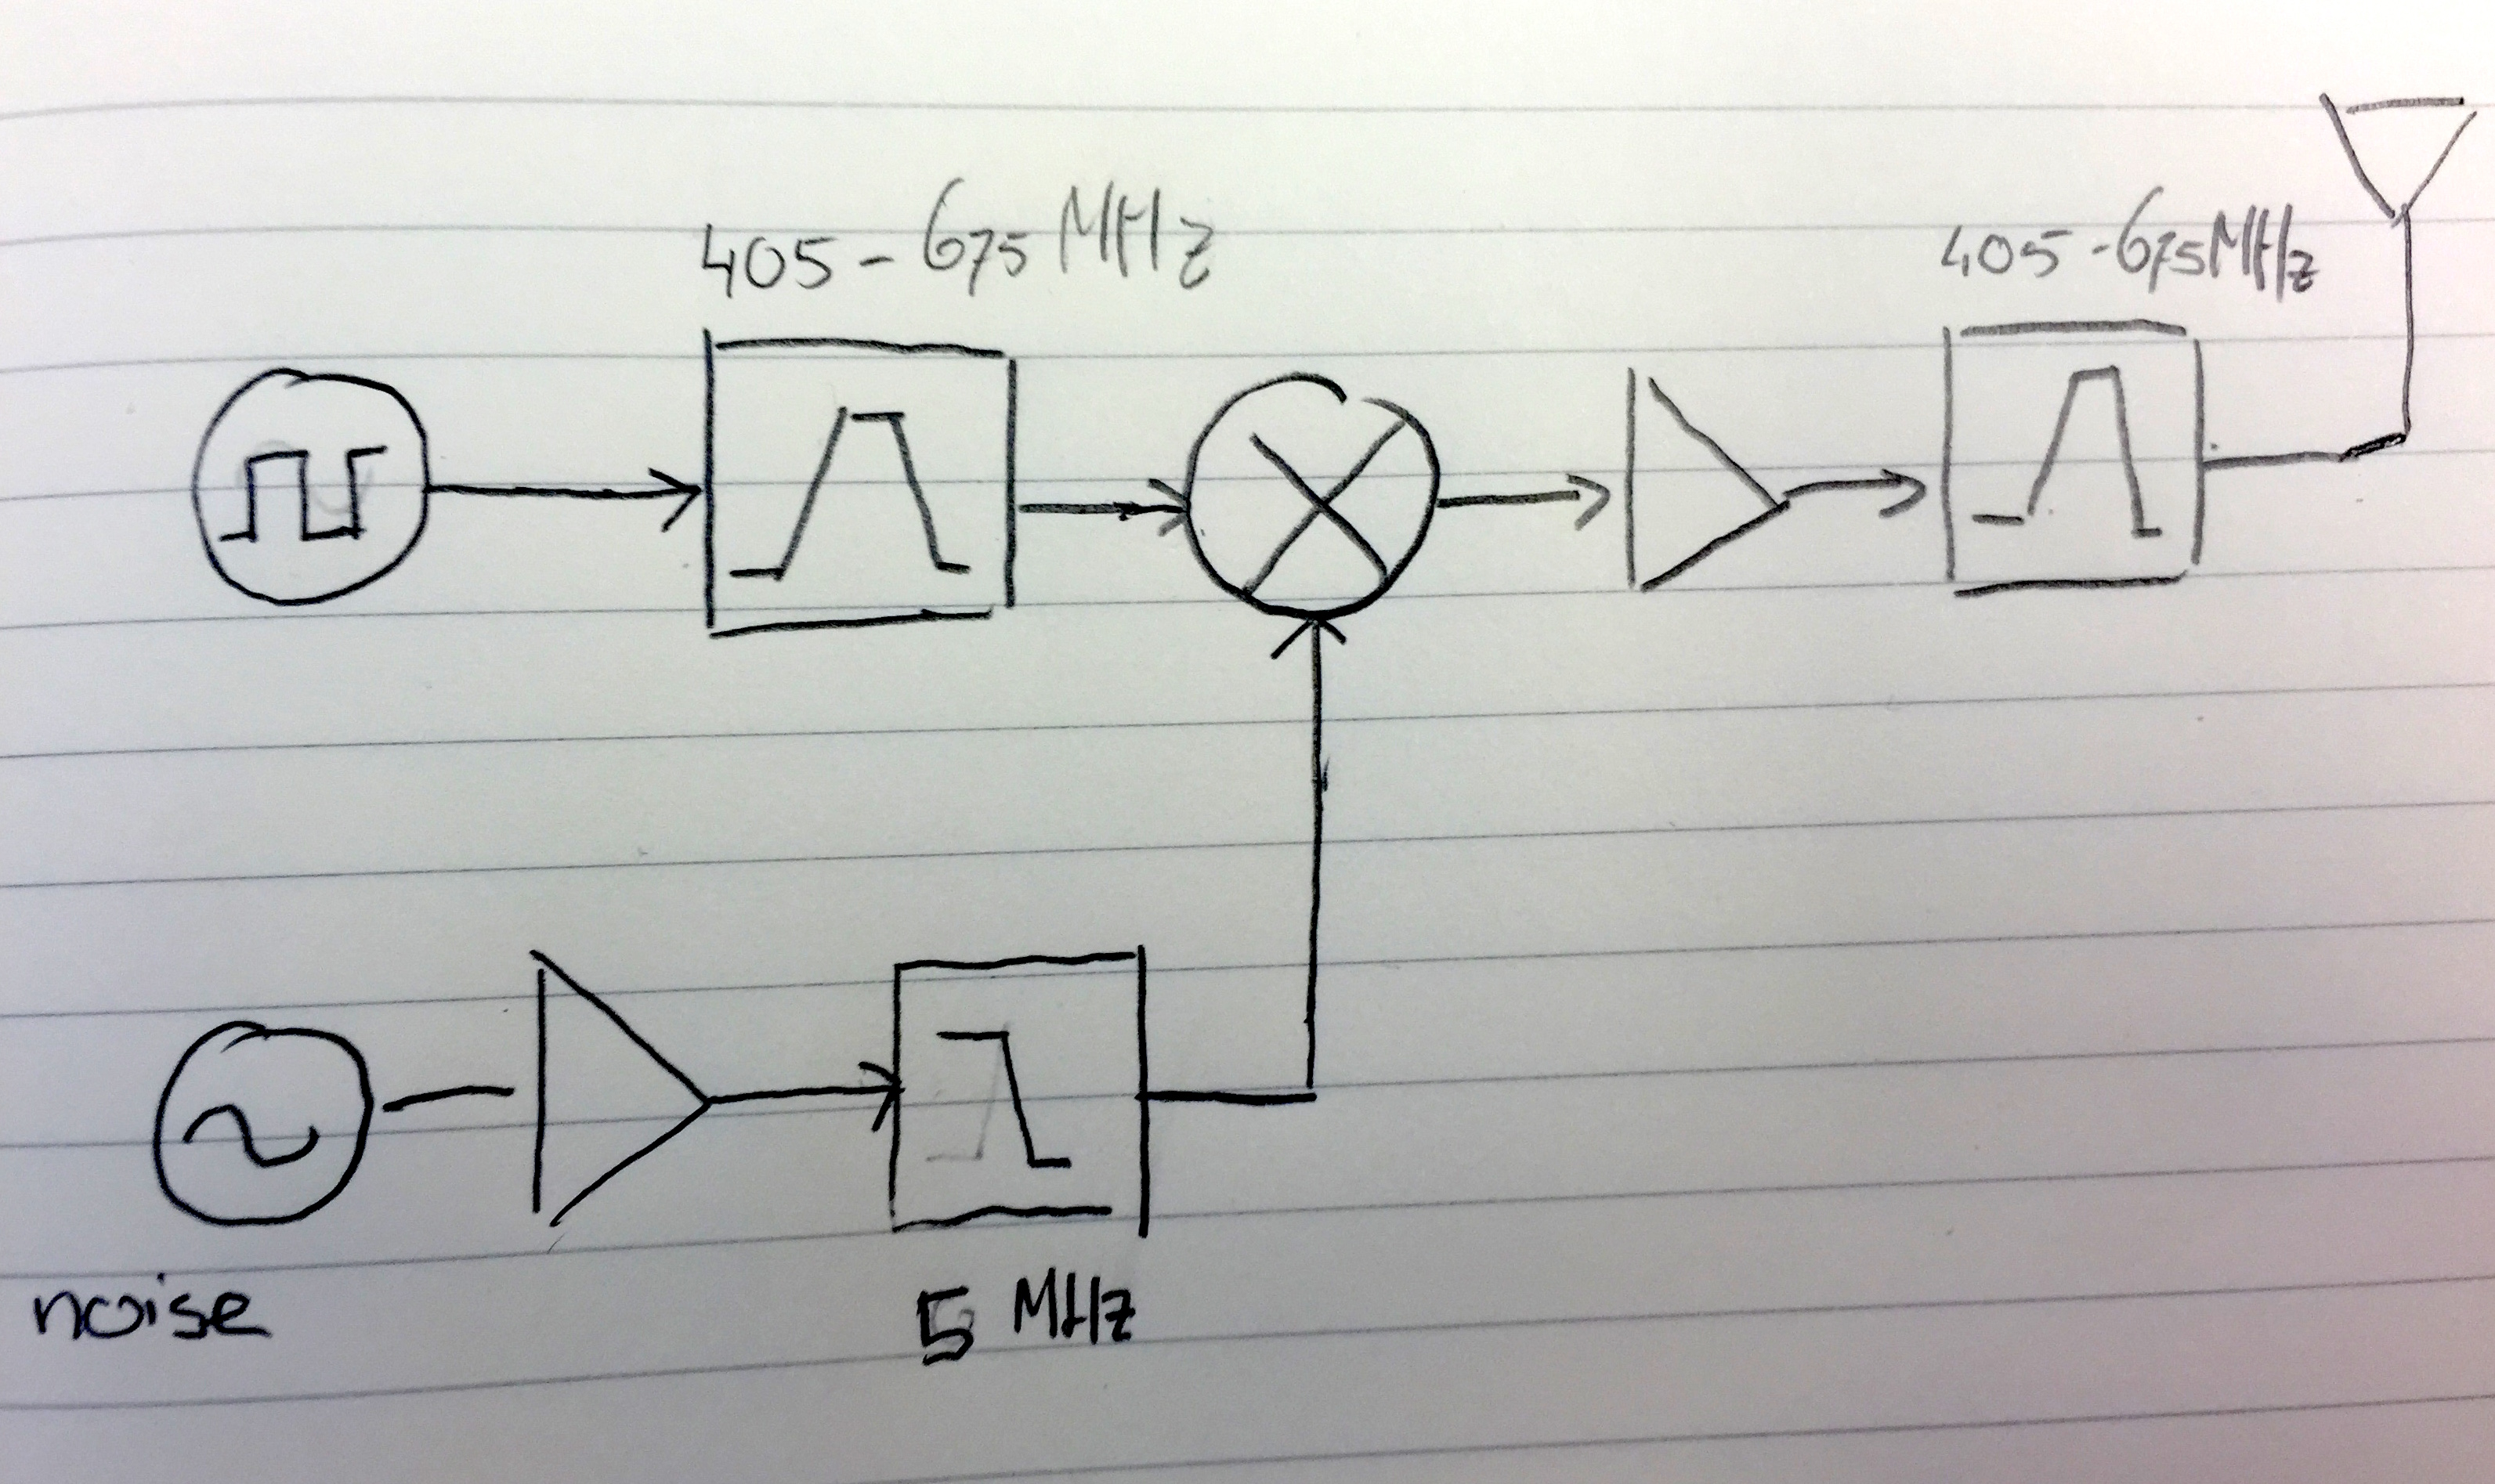
\includegraphics[width=\textwidth]{block_diagram.jpg}
    \caption{Block diagram of the jammer TODO: draw in tikz}
    \label{fig:block_diagram_jammer}
\end{figure}

The block diagram of the jammer can be found in \cref{fig:block_diagram_jammer}. The jammer works by generation a square wave with a programmable clock generator IC\@. These ICs are much cheaper than a solution with a very broadband voltage controller oscillator and a PLL\@. We chose a specific IC with a frequency range of \SIrange{3}{416}{\mega\hertz}. In this example we want to jam the band including the \SI{446}{\mega\hertz} frequency of licence free radios. Our oscillator only operates up to a frequency of \SI{416}{\mega\hertz}, therefore we need to select a high harmonic, in this case the third, and filter all of the other components of the square wave. In this case we use a bandpass filter that spans the \SIrange{405}{675}{\mega\hertz}. The bandwidth is determined by the frequency of the fifth harmonic. At \SI{405}{\mega\hertz} the base frequency is \SI{135}{\mega\hertz}, and the fifth harmonic \SI{675}{\mega\hertz}. We created a small script to generate a complete table of needed filters to span the whole range of \SI{3}{\mega\hertz} to \SI{3}{\giga\hertz}. These results can be found in \cref{tbl:filter_freqs}.

After that the filtered signal is mixed with a band-limited noise source, and then amplified and filtered again. This should produce a band limited signal with noise at the desired frequency.

\begin{table}[h]
\centering
\caption{Filter frequencies for frequency range of \SIrange{3}{3179}{\mega\hertz}}
\label{tbl:filter_freqs}
\begin{tabular}{rrrrr}
\toprule
   Harmonic &   Filter low [\si{\mega\hertz}] &   Filer high [\si{\mega\hertz}] &   LO low [\si{\mega\hertz}] &   LO high [\si{\mega\hertz}] \\
\midrule
          1 &            3 &            9 &        3 &         9 \\
          1 &            9 &           27 &        9 &        27 \\
          1 &           27 &           81 &       27 &        81 \\
          1 &           81 &          243 &       81 &       243 \\
          3 &          243 &          405 &       81 &       135 \\
          3 &          405 &          675 &      135 &       225 \\
          3 &          675 &         1125 &      225 &       375 \\
          5 &         1125 &         1575 &      225 &       315 \\
          7 &         1575 &         2025 &      225 &       289 \\
          7 &         2025 &         2601 &      289 &       371 \\
          9 &         2601 &         3179 &      289 &       353 \\
\bottomrule
\end{tabular}
\end{table}

\subsection{Schematics}
The schematics can be found in the appendix.


\subsubsection{Filter design}
For this implementation we chose a frequency range of \SIrange{405}{675}{\mega\hertz}. We designed\footnote{Designed with \url{http://www-users.cs.york.ac.uk/~fisher/lcfilter/}} a sixth order Chebyshev bandpass filter, with a ripple of \SI{1.0}{\decibel} in the passband, a characteristic impedance of \SI{50}{$\Omega$}. We also designed a matching network to match the \SI{50}{$\Omega$} of the filter to the \SI{180}{$\Omega$} input impedance of the mixer. The schematics of the filter can be found in \cref{fig:filter}.

\begin{figure}[h]
    \centering
    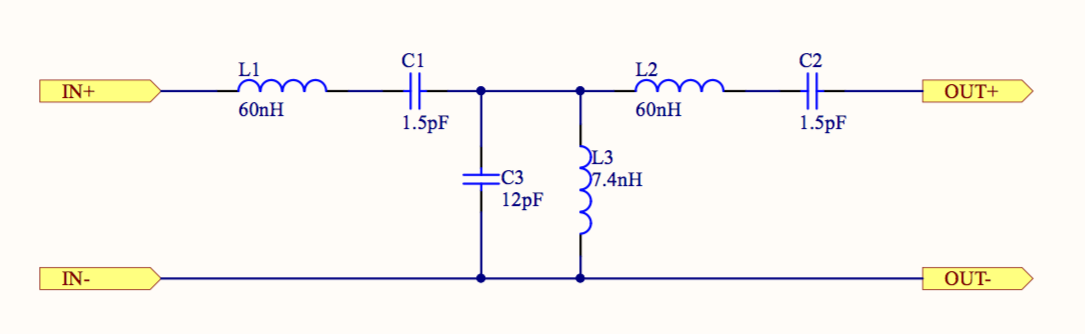
\includegraphics[width=\textwidth]{filter.png}
    \caption{The designed bandpass filter}
    \label{fig:filter}
\end{figure}

\subsubsection{Noise source}

\subsubsection{Microcontroller}

\subsection{Simulations}
To verify the working of the system we built a SPICE simulation of a simplified version of the schematic. We also simulated the filters to check if those were designed correctly.
\begin{figure}[h]
    \centering
    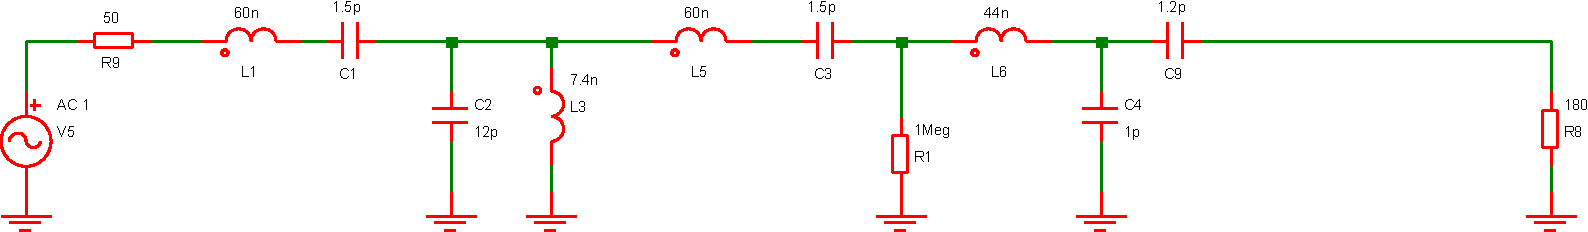
\includegraphics[width=\textwidth]{sim_schematic.pdf}
    \caption{Schematic of the filter and matching network used in the simulation}
    \label{fig:sim_schematic}
\end{figure}

\begin{figure}[h]
    \centering
    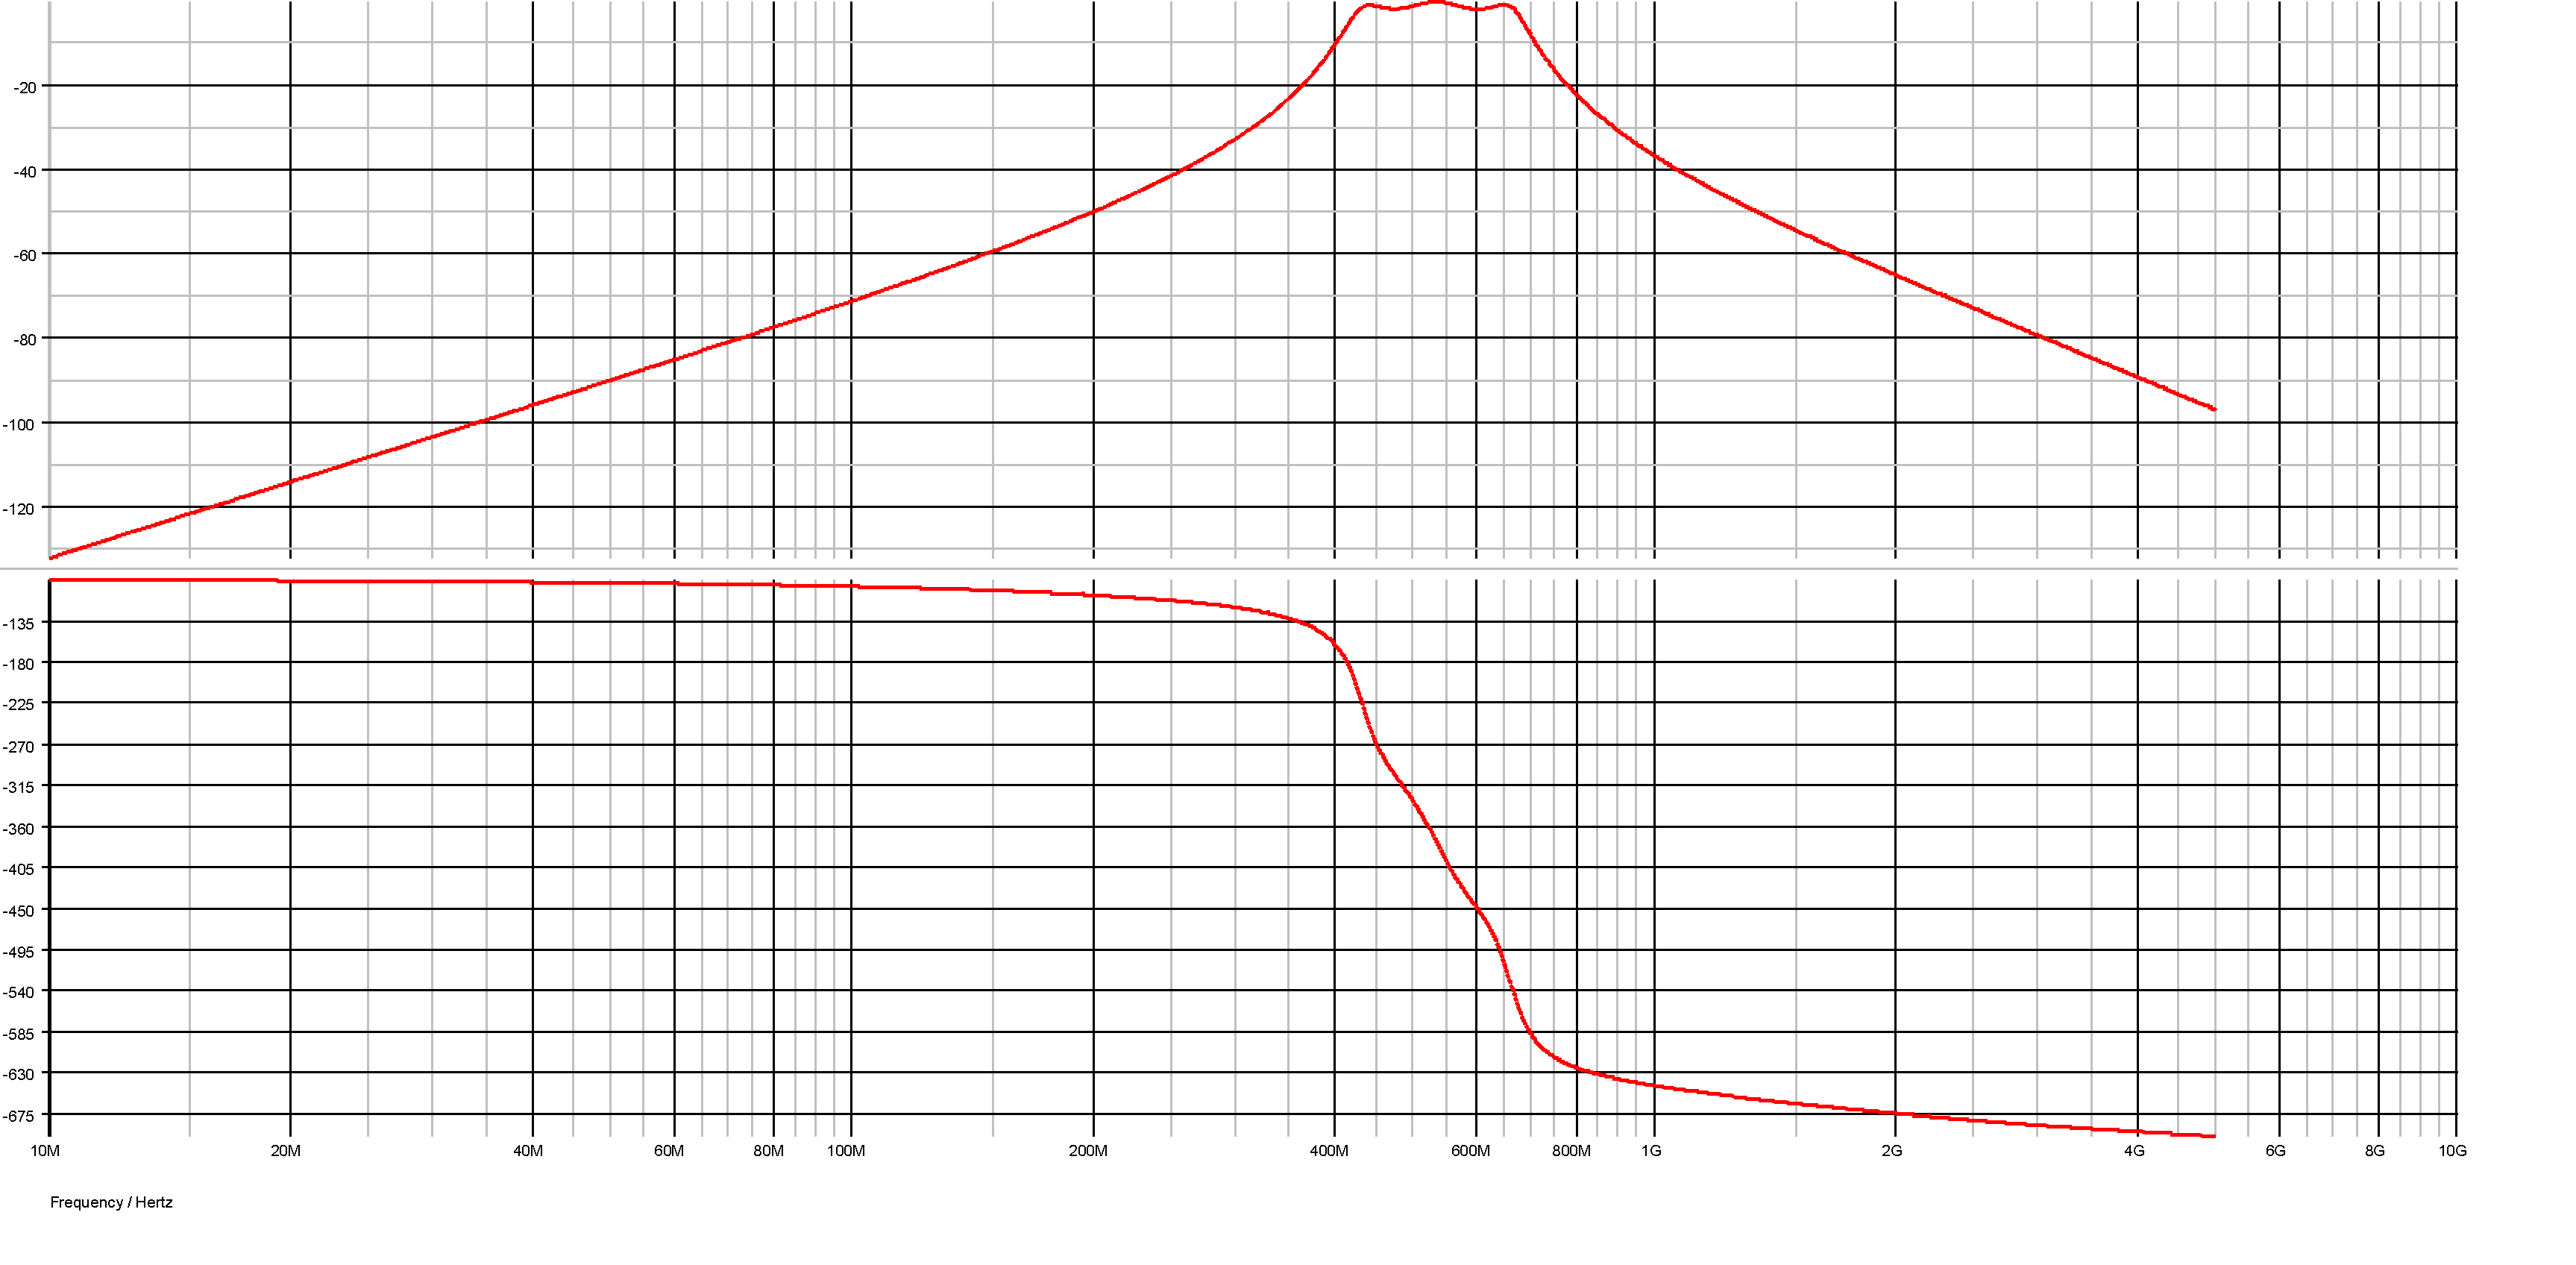
\includegraphics[width=\textwidth]{bode.pdf}
    \caption{Bode plot of the simulations}
    \label{fig:sim_bode}
\end{figure}





\subsection{Filters}




\subsection{PCB}
Coming soon\ldots

\begin{figure}[h]
    \centering
    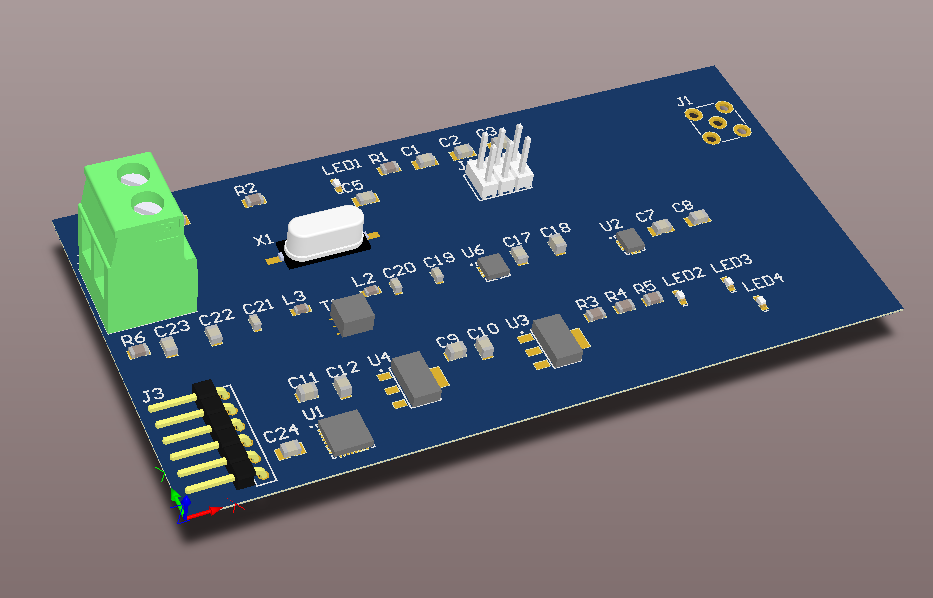
\includegraphics[width=\textwidth]{pcb.png}
    \caption{3D view of the designed PCB}
    \label{fig:pcb_3d}
\end{figure}

\end{document}
